% For OCCAM
% To be used for a0poster

\usepackage{graphicx}
\usepackage{color}
\usepackage{amsmath, amssymb, amsfonts}
\usepackage[absolute]{textpos}
\usepackage{url}

\pagestyle{empty}

% OCCAM colours definition
%
\definecolor{occamdark}       {rgb}{0.333,0.278,0.169}
\definecolor{occammedium}{rgb}{0.616,0.569,0.400}
\definecolor{occamlight}      {rgb}{0.890,0.863,0.596}
\definecolor{desert}          {rgb}{0.968,0.956,0.850} %HTML: f7f4d9
\newcommand{\bfb}{\bfseries\color{occamdark}}

% Set sizes and colours for textboxes (package: textpos)
%
\TPMargin{28pt}
\def\framethick{\TPshowboxestrue\setlength\TPboxrulesize{10pt}}

% swap these comments if you want frames around each text area
%\def\framethin {\TPshowboxestrue\setlength\TPboxrulesize{4pt}}
\def\framethin {\TPshowboxesfalse}

\def\frameoff  {\TPshowboxesfalse}

% Background colour
%
%\textblockcolour{desert}
\textblockcolour{white}
\textblockrulecolour{occammedium}

% Test sizes
%
\let\Textsize\normalsize

% if you have a longer title, you can use a smaller size here
%\def\Title #1{{\veryHuge\color{occamdark} \begin{center} #1 \end{center}}}
\def\Title #1{{\VERYHuge\color{occamdark} \begin{center} #1 \end{center} }}

\def\Head #1{\begin{center}\LARGE\color{occamdark} \textbf{#1}\end{center}\medskip}
\def\Subhead #1{\begin{center}\large\color{occamdark} \textbf{#1}\end{center}\medskip}
\def\Subsubhead #1{\color{occamdark}\textbf{#1}}

\parindent =0pt
\parskip   =0.5\baselineskip

% Columns: 4 cols of width 7 plus 3 gaps of width 1 (31=4*7+3*1)
%
\TPGrid[40mm,20mm]{31}{12} 
%\newenvironment{area1w}[1]{\TPMargin{40pt}\textblockcolour{white}\begin{textblock}{8}(-0.875,#1)}{\end{textblock}}
\newenvironment{area1}[1]{\textblockcolour{white}\begin{textblock}{7.75}(-0.75,#1)}{\end{textblock}}
\newenvironment{area2}[1]{\textblockcolour{white}\begin{textblock}{7.75}( 7.5,#1)}{\end{textblock}}
\newenvironment{area3}[1]{\textblockcolour{white}\begin{textblock}{7.75}(15.75,#1)}{\end{textblock}}
\newenvironment{area4}[1]{\textblockcolour{white}\begin{textblock}{7.75}(24,#1)}{\end{textblock}}




% Columns: 3 cols of width 10.333 (31=3*10.3333)
%
%\newenvironment{area1}[1]{\textblockcolour{white}\begin{textblock}{10.3333}(-0.6,#1)}{\end{textblock}}
%\newenvironment{area2}[1]{\textblockcolour{white}\begin{textblock}{10.3333}( 10.4,#1)}{\end{textblock}}
%\newenvironment{area3}[1]{\textblockcolour{white}\begin{textblock}{10.3333}(21.35,#1)}{\end{textblock}}
%%\newenvironment{area4}[1]{\textblockcolour{white}\begin{textblock}{7.75}(44,#1)}{\end{textblock}}

% To get a larger main body font, I inserted \large as follows (what
% is the "correct" way to do this with this poster class file?)
%\newenvironment{area1}[1]{\large\textblockcolour{white}\begin{textblock}{10.3333}(-0.6,#1)}{\end{textblock}}
%\newenvironment{area2}[1]{\large\textblockcolour{white}\begin{textblock}{10.3333}( 10.4,#1)}{\end{textblock}}
%\newenvironment{area3}[1]{\large\textblockcolour{white}\begin{textblock}{10.3333}(21.35,#1)}{\end{textblock}}



% Logos
%
\newcommand{\logos}{
\frameoff
%\begin{textblock}{0}(-.75,-0.3)
%
\includegraphics[width=270mm]{img/logo-occam}
%\end{textblock}
\begin{textblock}{0}(-0.95,-0.23)

\includegraphics[width=270mm]{img/logo-combined}
\end{textblock}
}
\newcommand{\logoscurves}{
\frameoff
\begin{textblock}{0}(19,9)

\includegraphics[width=470mm]{img/occam_banner_top_right}\\
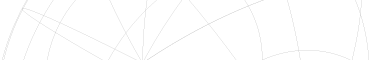
\includegraphics[width=470mm]{img/occam_banner_content_right}
\end{textblock}
}

% Hack to have a coloured background
%
\newcommand{\background}{
\framethick
%\frameoff
\begin{textblock}{33.26}(-1.13,-0.3)
\vspace{1.026\textheight}
\end{textblock}
}

% Hide References title
\renewcommand\refname{}
